\colorbox{white!10!}{
    \begin{minipage}{0.2\textwidth}
       \begin{flushleft}
        \includegraphics[width = 0.6\textwidth]{Эмблема.png}
       \end{flushleft}
    \end{minipage}
    \begin{minipage}[t]{0.7 \textwidth}
        \begin{center}
            {\huge \textsc{Красноярская Летняя Школа. Сезон $7^2 - 2$}}
            \vspace{0.25cm}
            
            { \huge \textbf{ФМТ. Свалка}}
        \end{center}
        \vspace{0.05cm}
    \end{minipage}
}

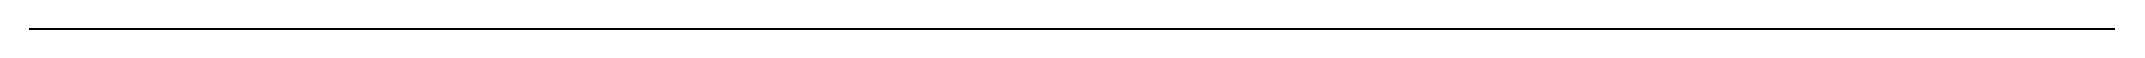
\begin{tikzpicture}
    \draw[thick] (-6.5,0)--(20,0);
\end{tikzpicture}
\begin{enumerate}
    \item К источнику последовательно через реостат подключен вольтметр. Если сопротивление реостата уменьшить втрое, то показания вольтметра возрастут вдвое. Во сколько раз изменятся показания вольтметра, если сопротивление реостата уменьшить до нуля?
    
    \parbox[b]{.7\textwidth}{
    \item 	К потолку и стенке ящика, находящегося на горизонтальной поверхности, подвесили груз массой $m$ на двух нитях. Нити составляют углы $\alpha$ со стенкой и $\beta$ с дном ящика, как показано на рисунке. Определить силы натяжения $T_1$ и $T_2$ обеих нитей, если известно, что система находится в равновесии.
	}\hfill\includegraphics[width=.3\textwidth]{pictures/Svalka.png}

\end{enumerate}